\documentclass{article}

% if you need to pass options to natbib, use, e.g.:
% \PassOptionsToPackage{numbers, compress}{natbib}
% before loading nips_2016
%
% to avoid loading the natbib package, add option nonatbib:
% \usepackage[nonatbib]{nips_2016}

\PassOptionsToPackage{numbers,sort&compress}{natbib}
\usepackage[final]{nips_2016} % produce camera-ready copy

\usepackage[utf8]{inputenc} % allow utf-8 input
\usepackage[T1]{fontenc}    % use 8-bit T1 fonts
\usepackage{hyperref}       % hyperlinks
\usepackage{url}            % simple URL typesetting
\usepackage{booktabs}       % professional-quality tables
\usepackage{amsfonts}       % blackboard math symbols
\usepackage{nicefrac}       % compact symbols for 1/2, etc.
\usepackage{microtype}      % microtypography
\usepackage{graphicx}
\usepackage{caption}
\usepackage{subcaption}
\usepackage{txfonts}
\usepackage[parfill]{parskip}
\usepackage[font=small,labelfont=bf]{caption}
\setlength\parindent{0pt}

\title{World Wide Trends in Spotify}

% The \author macro works with any number of authors. There are two
% commands used to separate the names and addresses of multiple
% authors: \And and \AND.
%
% Using \And between authors leaves it to LaTeX to determine where to
% break the lines. Using \AND forces a line break at that point. So,
% if LaTeX puts 3 of 4 authors names on the first line, and the last
% on the second line, try using \AND instead of \And before the third
% author name.

\author{
  s2306209\\
  %% examples of more authors
  \And
  s2435255\\
 \And
  s2340198\\
}

\begin{document}

\maketitle

\begin{abstract}
 In this report we are mainly focusing on predicting the region and popularity of the Track based on its features, Track name and Artist name. The calculated popularity index gives us the popularity of the Track considering important factors such as the total number of streams, frequency and age of the song. The popularity prediction is done in two different methods, one using the calculated popularity score using regression models and the other based on the most popular tracks per region using binary classification. The region prediction is achieved using classification models. The classification problems are done with the help of Naive Bayes, KNN, Decision Trees and Random Forest and the Regression problem is implemented through Decision Trees, Random Forest and Linear Regression. It is observed that random forest gives the best accuracy in both the classification and regression problems.   
\end{abstract}

\section{Introduction}

Spotify is a well renowned music streaming platform which has gained great momentum in the recent years. Since its establishment in the year 2006 in Sweden the music platform has been used all over the world. It was observed that Spotify even though didn't start with great profits \cite{setty2013hidden}, reached great heights with respect to cultural regions by offering a number of multilingual music and genre. In this report we will be discussing and predicting the popularity of a song based on region, predicting the region of the song based on the song features and the correlation between the popularity of a song with respect to another region. There are limited previous publications which perform a similar analysis. From the research paper that we found relevant \cite{9776765} the song features such as dance-ability and tempo are being used to find the popularity of the song.

There are multiple applications of predicting the popularity of a song based on a region, as knowing the average reach of a song is a primary requirement in the music industry. This will help the music composers and the producers check the reachability and the popularity of a song beforehand and the factors that contribute towards this. Our concept will also help in understanding which is the most optimal region in which the song will be most played hence being the most popular.

\section{Data Preparation}

\subsection{Data Collection}
The given dataset only comprises of the track names, artists, streams, URL, date and region. It was tough to get the required predictions based on just these features. Hence we extracted the Track ID from the URL of the tracks and obtained the song features using "Spotipy" which is a lightweight Python library for the Spotify Web API. Given below are the extracted song features and their meaning:

\begin{itemize}
    \item Danceability: This tells us how suitable the song is for dancing. It varies between a range of 0.0 to 0.1, 0.0 being the least danceble and 1.0 being the most.
    \item Energy: This gives us the perceptual measure of intensity and activity. This ranges between 0.0 to 1.0. Mostly these kind of tracks are loud, fast and noisy.
    \item Tempo: This gives the overall estimated beats of a track per minute. tempo is the speed or pace of a given piece and derives directly from the average beat duration.
    \item Valence: This projects the musical postiveness. 1.0 being songs which are more cheerful and happy where as 0.0 gives us more negative songs.
    \item Key: This gives the average key of the overall song
    \item Loudness: This is a measure of the overall loudness of the track in decibels. It ranges between 0 to -60.
    
\end{itemize}

\subsection{Data Preprocessing}

We are provided with a dataset which consists of 3440540 rows and 7 columns. To this we added more features (columns) as mentioned earlier. This was achieved using "Spotipy" by applying an inner join on the track Ids which were obtained. Since a few songs were not present the size of the dataset reduced to 3440521 rows and 17 columns. After this we made separate columns for day, month and year using the date of the track. 

Track popularity was calculated after this. After applying multiple formulae we settled on the one that worked the best. This factors in the Region's cumulative song streams, frequency of the song in the region and the age of the song based on its first appearance in the dataset as shown in Equation (1). The final calculated track popularity is inserted into the existing dataset.   

\begin{equation}
    Popularity Index (Region) = \frac{Total Number Of Streams in the Region}{Frequency Of the Song in the Region} * Age of the song
\end{equation}


\section{Exploratory Data Analysis}

Using the data from preprocessing step, we checked the relation between the streams and region in-order to check which regions have the maximum and minimum number of streams. We also plotted a graph to observe the trends of streams for days of the week.

From the data we took the top 25\% songs in each region based on the streams as popular songs. We calculated the total streams of popular songs and the total streams in each region and plotted it in a bar graph as shown in Figure \ref{fig:Barplot}. This shows that the top 25\% songs cover most of the streams in every region. Hence we assume the top 25\% songs as popular while the rest as not popular for each region.
We have only shown the top 10 regions in the graph for analysis and visualisation purposes. The other regions in the dataset also followed the same pattern.

\begin{figure}[htbp]
    \centering
    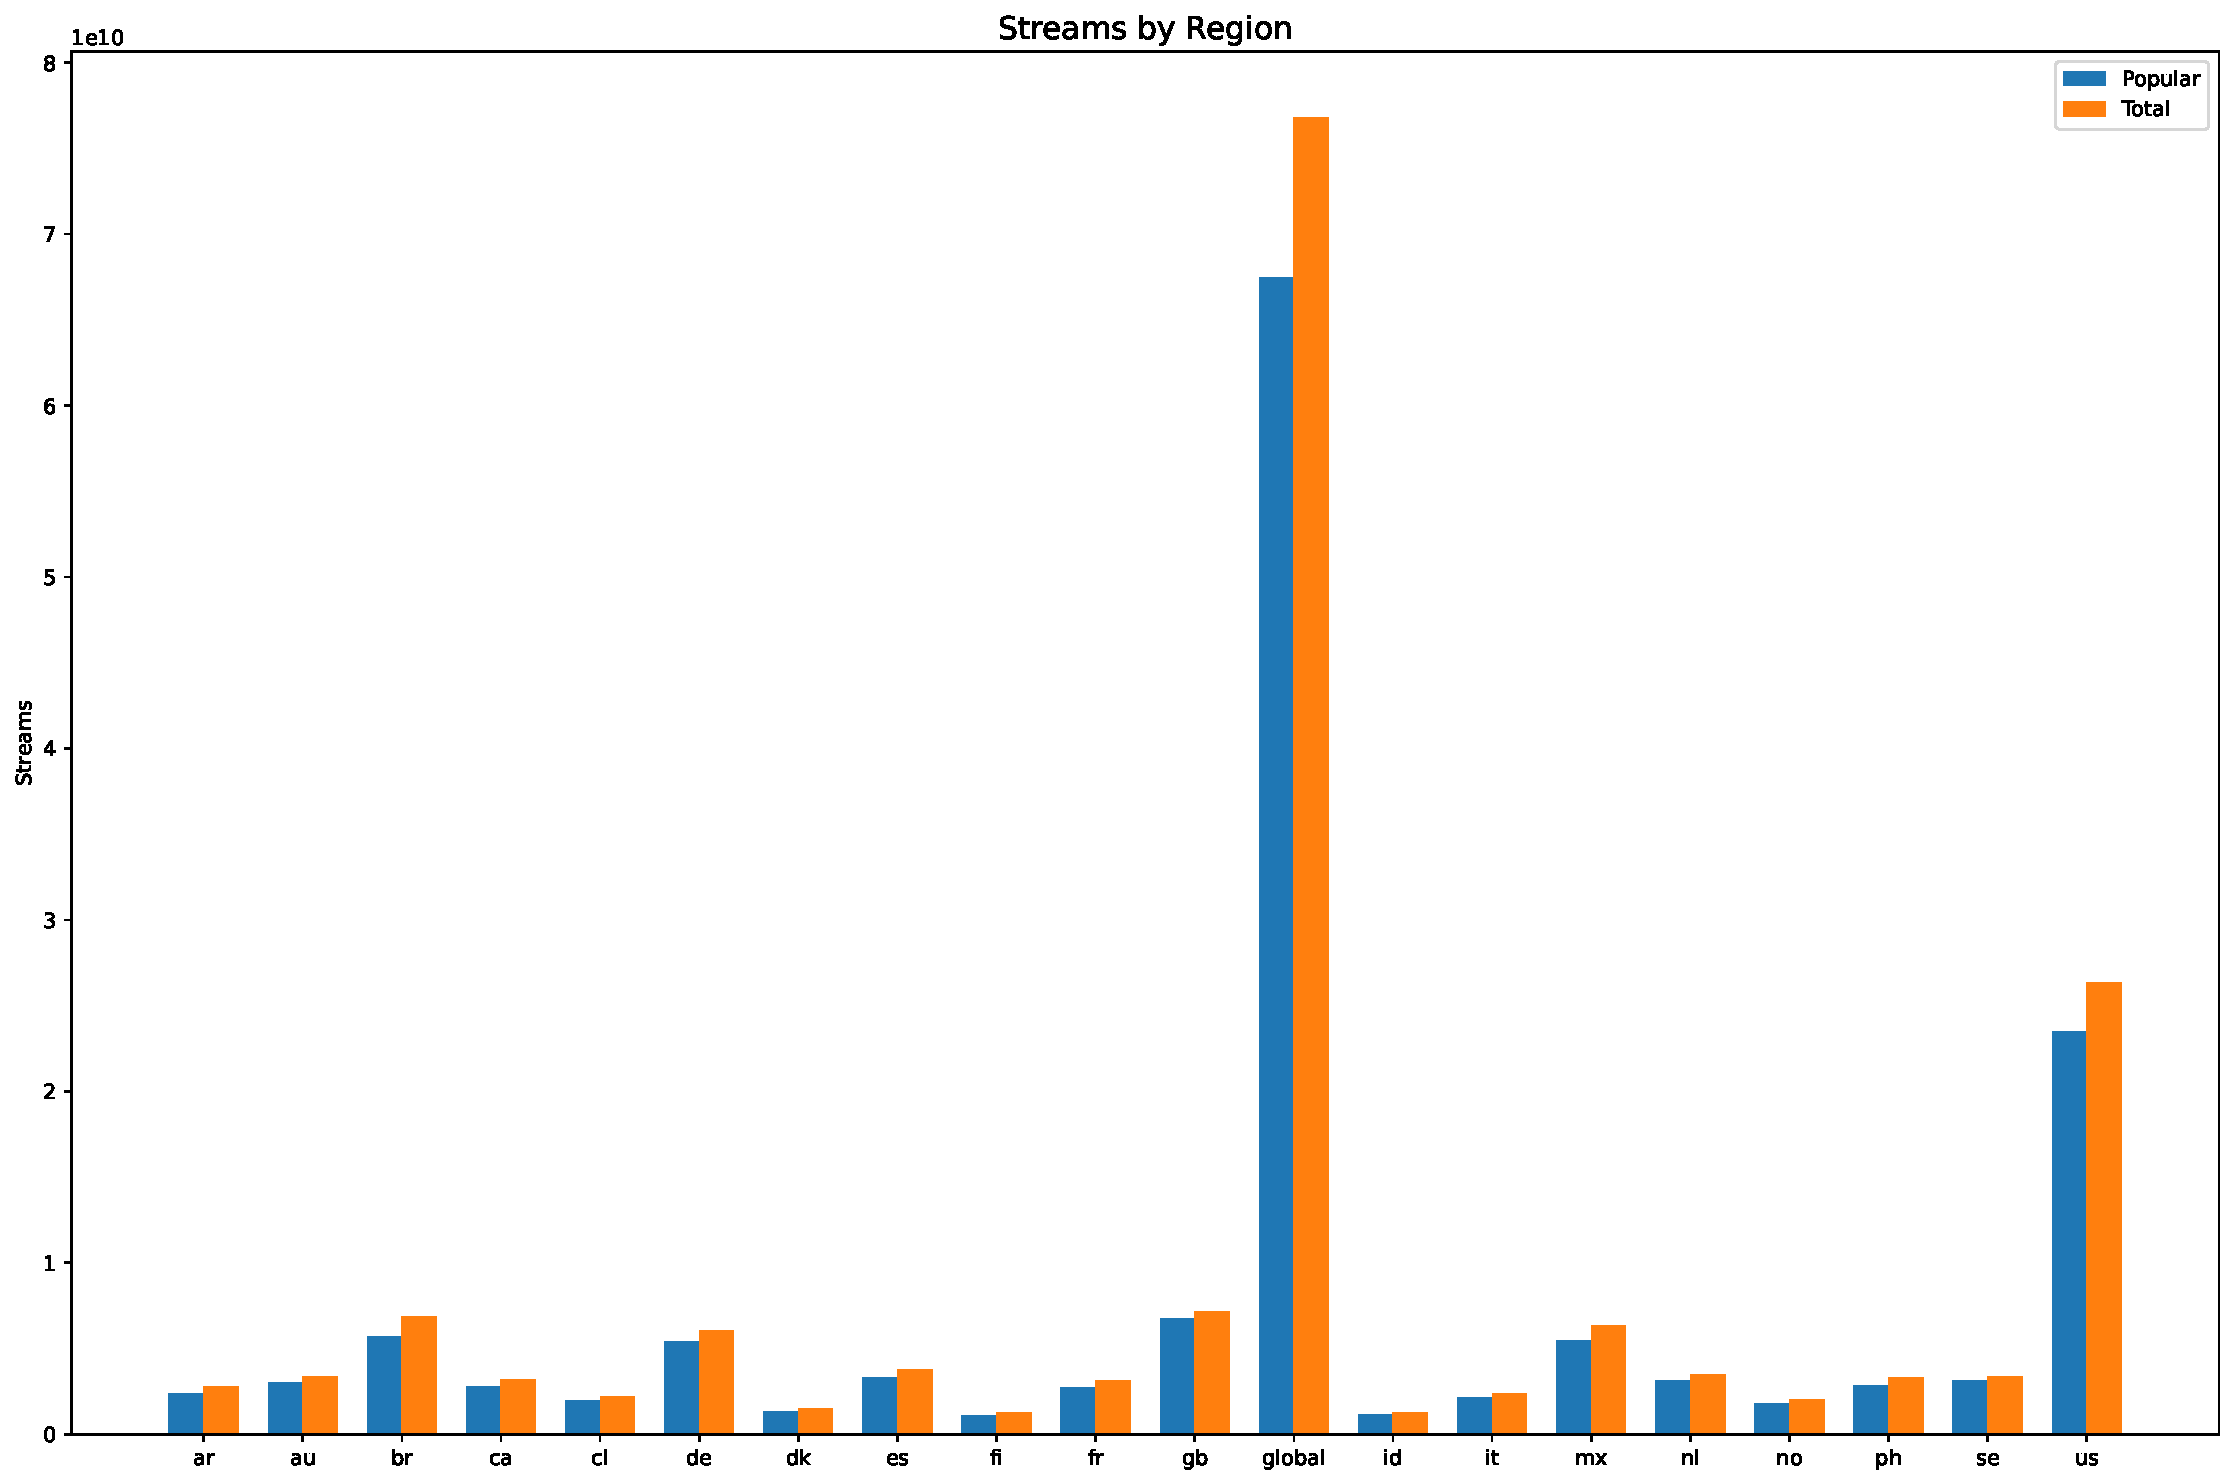
\includegraphics[scale = 0.25]{Figures/Region_streams.pdf}
    \caption{Bar plot representing the trends in streams across regions}
    \label{fig:Barplot}
\end{figure} 

Correlation matrix was calculated after this to check the correlation between the song features and the track popularity and streams as seen in Figure \ref{fig:Heatmap}. From the matrix it is noticed that energy is highly correlated with loudness hence one of these features can be dropped. Therefore we will be dropping energy from our dataset for further calculations

\begin{figure}[htbp]
    \centering
    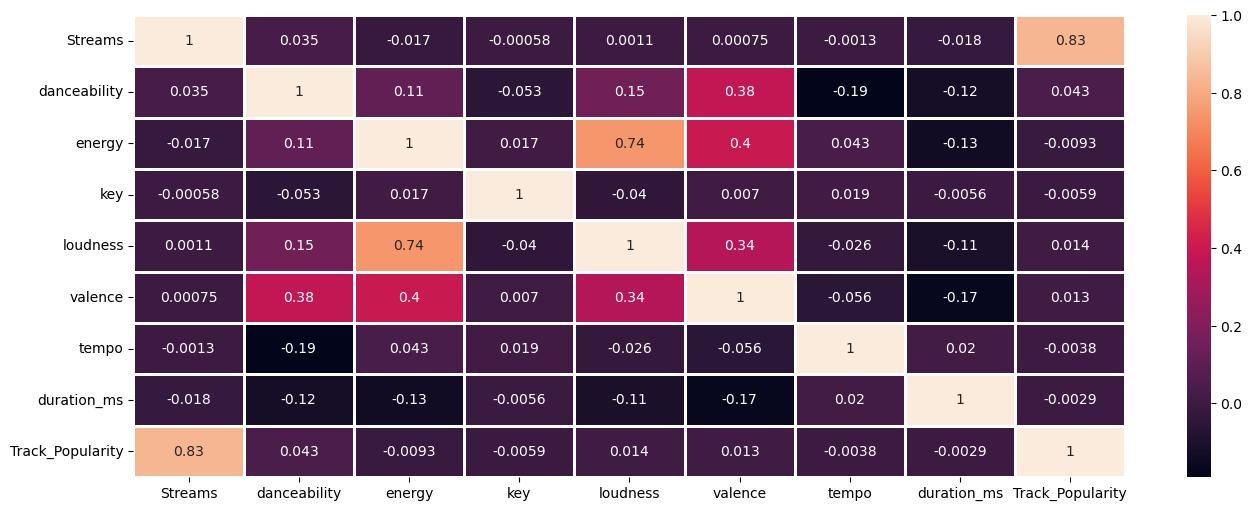
\includegraphics[scale = 0.40]{Figures/corrMatFeatures.jpeg}
    \caption{Correlation Heatmap: The figure shows a correlation heatmap with the song features and the calculated Track popularity}
    \label{fig:Heatmap}
\end{figure} 

\subsection{Impact of popularity on one region in comparison to another}
Another correlation matrix was formulated to check the correlation between the popularity of a song in one region with respect to another region. This was achieved with the region wise popularity index which was calculated and inserted into the dataset. The figure \ref{fig:corrRegion} in Appendix\ref{appendix:a} shows the mentioned matrix. For example we can see some examples like Germany (de) and Austria (at), Malaysia(my) and Singapore(sg) are highly correlated from the matrix. This shows that a popularity of a song in one region can affect the popularity in the other region which are highly correlated.

\subsection{Encoding}
Manual encoding was done for Track name, Artist name and Region to train the data in the model. Manual encoding for this was achieved with the help of running a loop to convert the names to numbers based on counter.

\section{Methodology}



In this report we will be taking up two research questions as stated before. 

\subsection{Models used:}
\begin{itemize}
    \item K-Nearest Neighbour: Also known as KNN is a non parametric, supervised classifier. This classifier uses proximity to classify or predict an individual data point. The K value is an integer. Depending on this K value the data point will be compared against K number of nearest data points based on proximity and will be classified appropriately. 
    
    \item Decision Tree Classifier: Decision Tree classifier is a supervised classification model with a tree like structure. The model consists of nodes and leaves. When a data point enters it is tested against the condition on the node and then classified according to the satisfied condition.
    
    \item Random Forest Classifier: Random Forest Classifier is nothing but an ensemble learning method. This is a group of decision trees for better classification by cross validating the subsets of the dataset hence reducing the overfitting problem and increasing accuracy.
    
    \item Linear regression: Linear Regression is the supervised Machine Learning model in which the model finds the best fit linear line between the independent and dependent variable i.e it finds the linear relationship between the dependent and independent variable.
    
    \item Naive Bayes: Naive Bayes is a classification algorithm for binary (two-class) and multi-class classification problems. The technique is easiest to understand when described using binary or categorical input values.
    
    \item Decision Tree Regressor: The Decision Tree Regression works the same way as the Decision Tree classifier. The only difference is that regression models are used for continuous data.
    
    \item Random Forest Regressor: Same as Random Forest classifier. But the Regressor works for continuous data. 
\end{itemize}

All the models were ran using the python sklearn library.


\subsection{Popularity Prediction}

\subsubsection{Classification - Using Naive Bayes, Decision Tree, Random Forest}
For this problem statement we have implemented binary classification by segregating the data as popular and not popular. This classification is done by finding the top 25\% most streamed songs per region and as seen earlier in figure \ref{fig:Barplot}   these top 25\% songs contribute the most to the total number of streams in that region. The obtained top percent is being considered as popular denoted with a value of 1 and the rest of the songs are assigned a value of 0 stating that they aren't popular. 
Then we've run classification based on artist and the song features (i.e. danceability, key, loudness, valence, tempo, duration\_ms). Then we've run the the classification using Naive Bayes. And then decision tree and random forest classifiers were utilised with depths ranging from 1 to 30 to find the best fitting model. 

\subsubsection{Regression - Using Linear, Decision Tree, Random Forest}
For this problem statement we used the popularity score calculated to run the regression model. First we found the total number of streams of a track per region. Then we've run the regression model based on artist, total number of streams of track per region and song features (i.e. danceability, key, loudness, valence, tempo, duration\_ms) to predict the popularity score. Initially, linear regression was used to train the data after which decision tree and random forest regressors were run with depths ranging from 1 to 30 to find the best fitting model. 

\subsection{Region Prediction - Using KNN, Decision Tree and Random Forest classification}

In this we have used features Position, Artist Name, Track Name, Day, Month, Streams, and song features (danceability, key, loudness, valence, duration\_ms, tempo) for predicting which region the song belongs to. Three classification models were used for this problem statement.
First, we  ran the KNN model which gave similar accuracy at lower k values in the range of 1-5. Increasing the k-neighbours value to 100 decreased its accuracy.
Next we ran the Decision tree model with varying depths of 10,20,30,40 and 50 to find the best fitting model.
Random Forest classifier was run after this at depth 20, which gave the best accuracy. 


\section{Evaluation \& Results}


\subsection{Popularity Prediction}


The Figure \ref{fig:ScoresBarPlotPopularityPredict} depicts the variations in classification scores across different models that were used. From this it is evident that Random Forest Classifier performed the best for this problem statement. We used 10 fold cross validation across 3 different training models which predicts the popularity of the song based on song features and artist to test over this. The dataset is split into 75\% training data and 25\% testing data to train the classification models and it is split 70\% training data and 30\% testing data for regression models.


\begin{figure}[!ht]
    \centering
    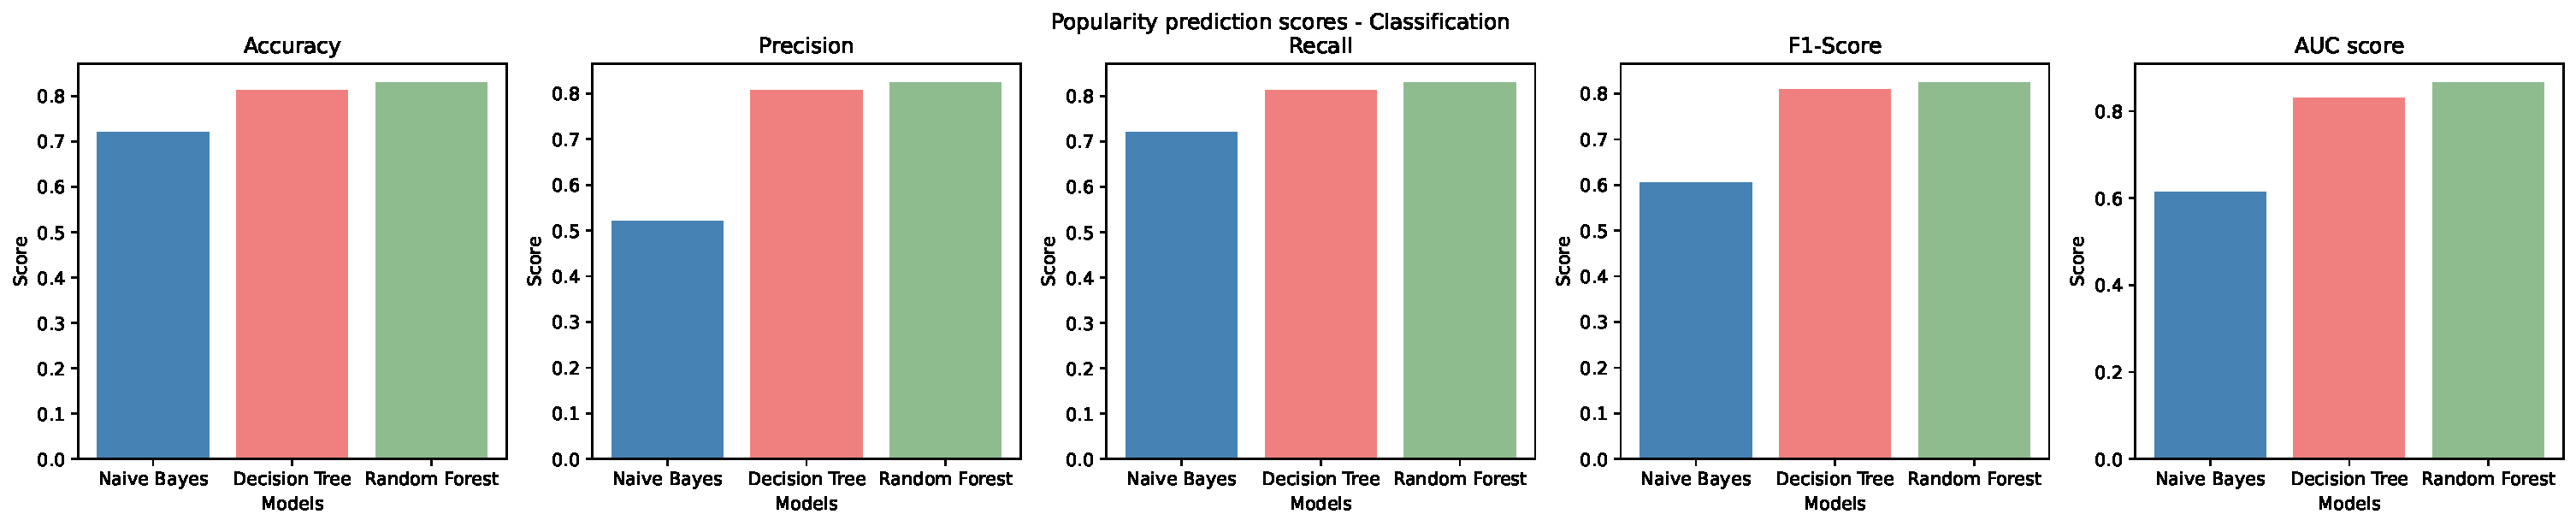
\includegraphics[width=\linewidth]{Figures/Popularity_prediction_scores_Classification.pdf}
    \caption{Popularity Prediction Scores (Accuracy, Precision, Recall, F1-Score and AUC-ROC) over cross validation dataset for classification problem}
    \label{fig:ScoresBarPlotPopularityPredict}
\end{figure} 


The figure \ref{fig:accuracylossplot} performs grid search across different depths ranging from 1 to 30 for decision tree regressor \& classifier and random forest regressor \& classifier. The model fits best at depth of 9 for decision tree classifier, at 12 for random forest classifier, at 6 for decision tree regressor and at 6 for random forest regressor. We can observe from the plots that after this particular depths the gap between training and validation loss increases which causes overfitting. 

\begin{figure}[!ht]
    \centering
    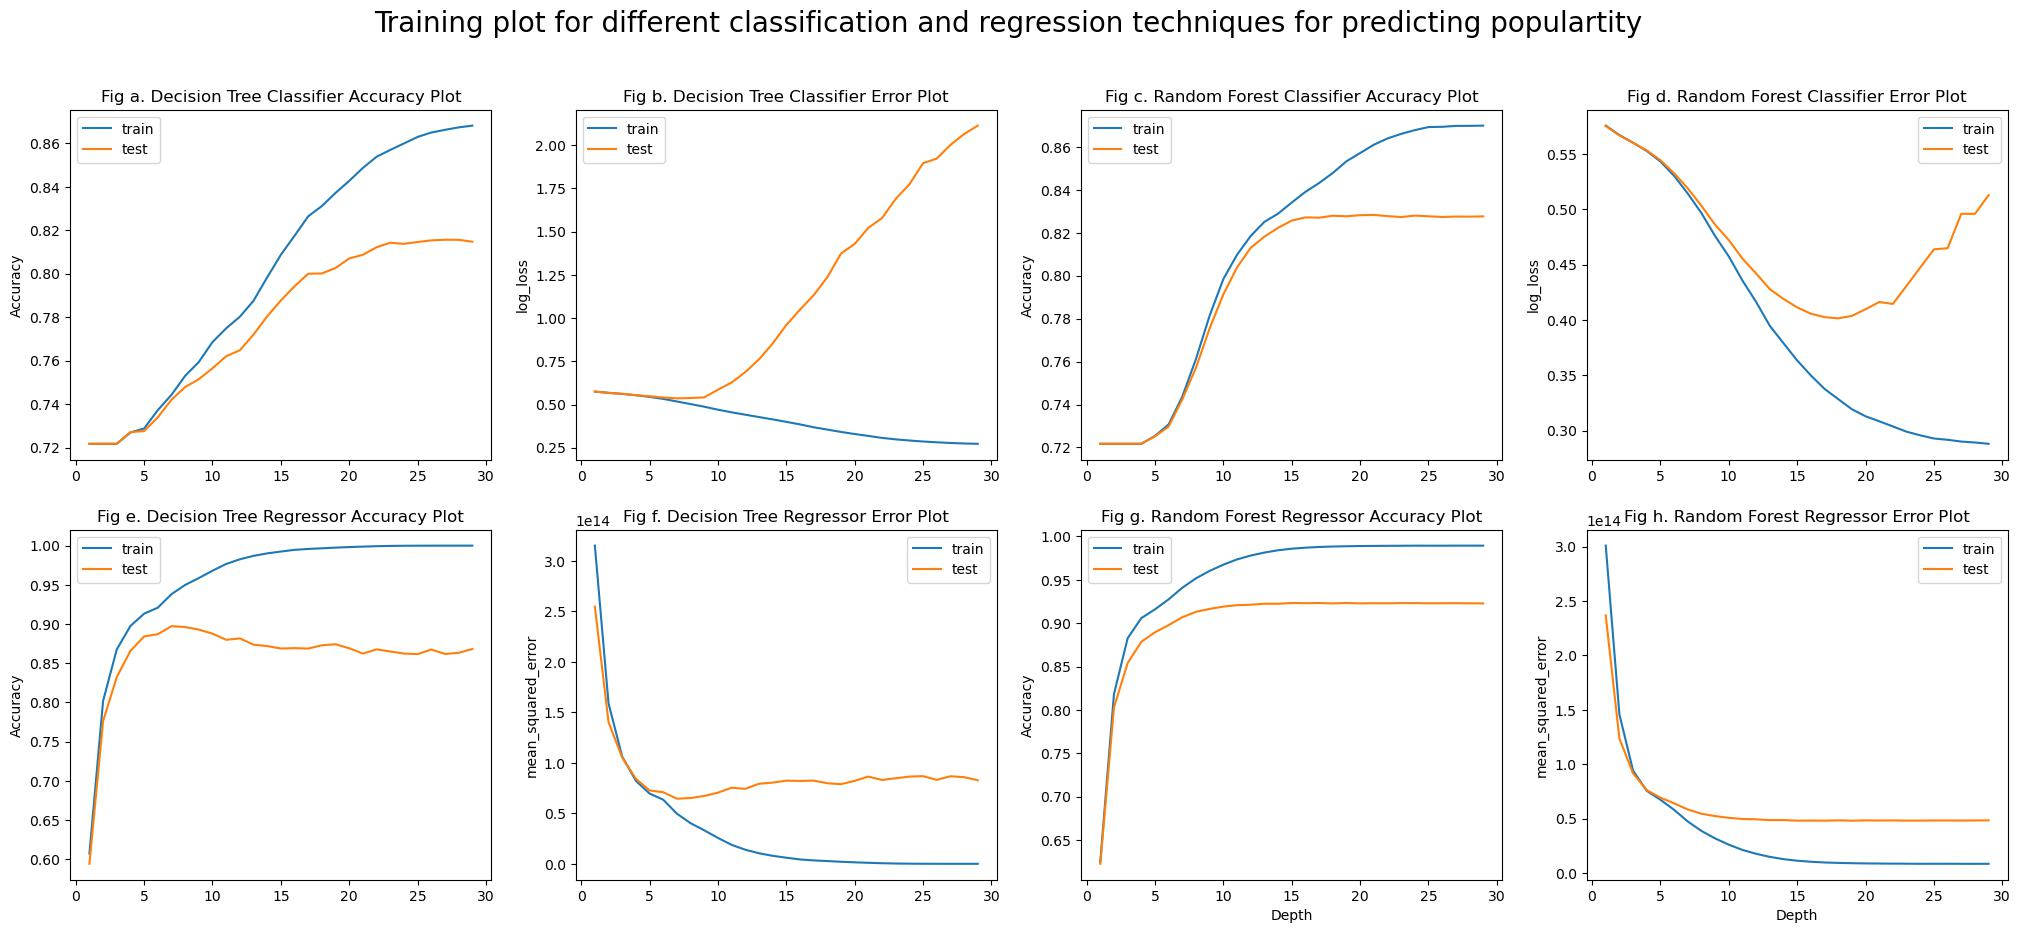
\includegraphics[scale = 0.25]{Figures/Popularity_accuracy_loss_plot.jpeg}
    \caption{Training and Testing curves for Decision Tree and Random Forest for predicting popularity}
    \label{fig:accuracylossplot}
\end{figure} 

\subsection{Region Prediction}

The Figure \ref{fig:regionPredClassReport} depicts the variations in scores across three different models. From the figure it can be concluded that random forest classifier obtained the best results for the problem statement. 3 fold cross validation was used across the models which predicts the region of the song based on song features, Track name and artist name. The training data is split into 80\% training data and 20\% testing data to train the models.

The Figure \ref{fig:decisonTreePlotsRegionPred} depicts grid search for Decision tree. It plots the accuracy and log loss error at tree depth of 10, 20, 30, 40, and 50. It can be seen that the test accuracy increases and log loss decreases till tree depth of 20. After this point the training loss keeps on decreasing while the test loss starts to increase. Hence the model overfits from this point onwards. It performs very well on the training data but does not generalise well on unseen data.
Therefore we choose tree depth value of 20 for predicting the region.

\begin{figure}[!ht]
    \centering
    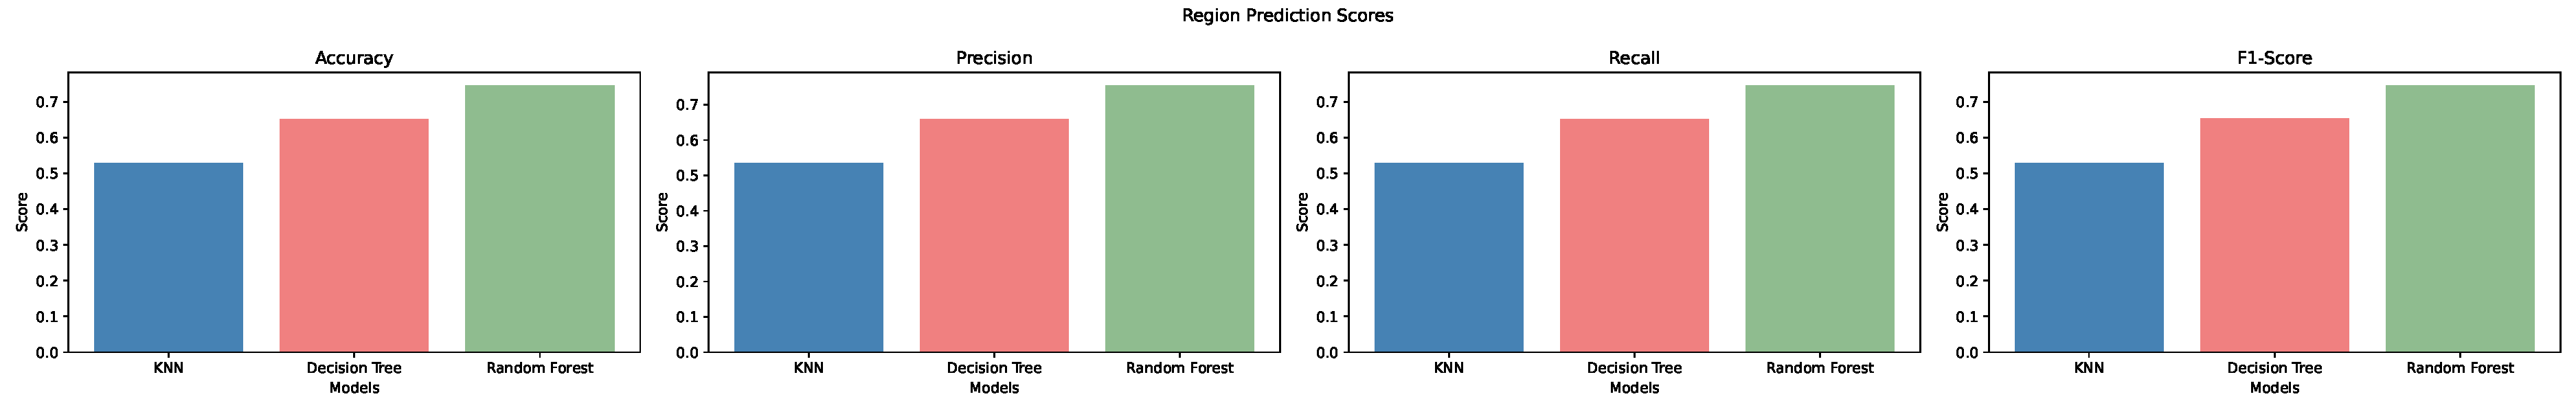
\includegraphics[scale = 0.24]{Figures/Region Predictions (1).pdf}
    \caption{Region Prediction Scores (Accuracy, Precision, Recall and F1-Score) over cross validation dataset for classification problem}
    \label{fig:regionPredClassReport}
\end{figure} 

\begin{figure}[!ht]
    \centering
    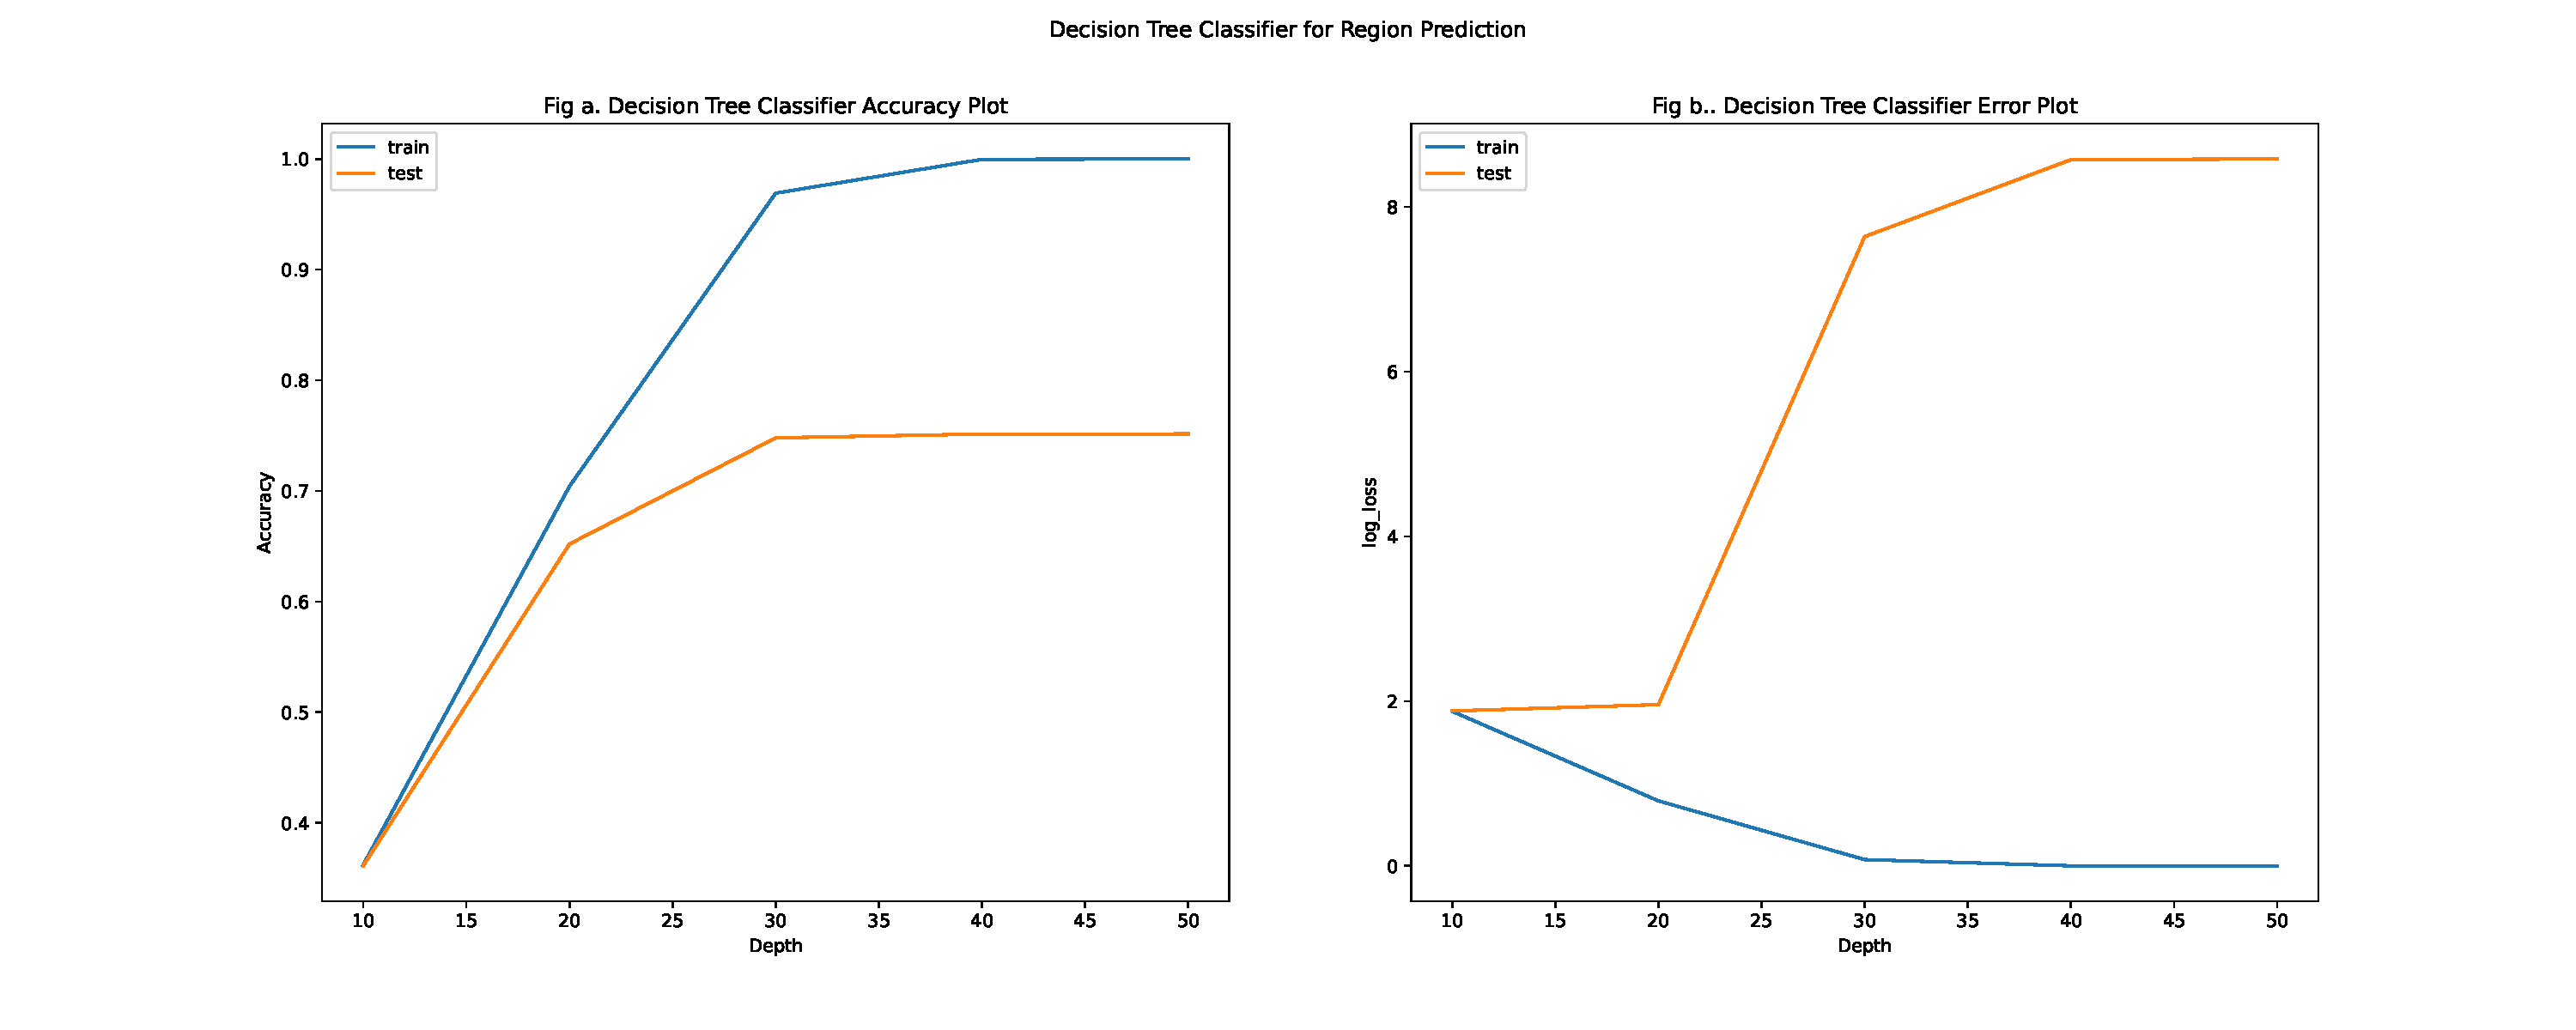
\includegraphics[scale = 0.20]{Figures/Region.pdf}
    \caption{Training and Testing curves for Decision tree for Region Prediction}
    \label{fig:decisonTreePlotsRegionPred}
\end{figure} 

\begin{table*}[t]
    \centering
    \begin{tabular}{|lr|lr|lr|}
    \toprule
        Popularity                   & Classification   & \ Popularity                   & Regression   & \ Region & Prediction \\
    \midrule
        Model & Accuracy & Model & Accuracy & Model & Accuracy \\
        Naive Bayes & 60.5 & Linear Regression & 84.5 & KNN & 52.9\\
        Decision Tree & 80.8 & Decision Tree & 88.6 & Decision Tree & 65.2\\
        Random Forest & 82.3 & Random Forest & 89.7 & Random Forest & 74.5\\
    \bottomrule
    \end{tabular}
    \caption{Accuracy for classification and regression models on Test Data}
    \label{tab:table_accuracy}
\end{table*}




\section{Conclusion}

In this research we have considered multiple different factors which influence the popularity of the track and the features which influence the region as well. The popularity prediction is done in two different methods, one that uses the popularity score calculated by region and the other which uses binary classification. For the binary classification, we analyse the data such that the top 25\% of the songs based on streams per region are considered to be popular with a popularity index as 1 and the rest as 0. 1 meaning popular and 0 meaning not popular. On further exploring this popularity index multiple classification models are applied to check which factors influence the popularity of a track. The region prediction is done with the help of song features, Track Name and Artist name. It is noticed that in a few cases the artist's name influences the popularity of a song in few regions. It was observed that random forest regressor and/or classifier produced the best results in all the cases. The accuracy can be seen in the Table \ref{tab:table_accuracy}

The Track features which were obtained using Spotify's Web API proved to be useful in predicting both the region and the popularity. Nevertheless, it was also observed that some of these features don't add much to these predictions through a correlation matrix. After multiple permutations and combinations we settled on a few features which influenced the prediction scores to a noticeable extent. Since the data obtained from Spotify is quite limited, better results could be achieved if more features can be obtained \cite{inproceedings}.

The results can be better obtained with respect to regions if we could also get the population of a region as this would influence this vastly. It can be assumed that, regions with larger population will have more streams in comparison to the smaller regions. 





\section*{Citations and References}

\bibliography{refs.bib}
\bibliographystyle{plain}

\section*{Statement of Contribution}

The ideology behind the project was developed after multiple team meetings and group discussions. We finally decided upon the problem statements and began to work. Since we had three problem statements, we split it amongst each other. Popularity prediction was contributed mostly by s2340198 and s2306209 and Region prediction was contributed majorly by s2435255. Nevertheless, we all helped each other out throughout the duration of the project whenever we got stuck or in requirement of an idea to proceed further. The report writing was a group effort and everyone contributed equally towards this.  

\section*{Appendices}
\appendix

\section{Correlation matrix: Correlation between popularity of tracks across regions}
\begin{figure}[!ht]
    \centering
    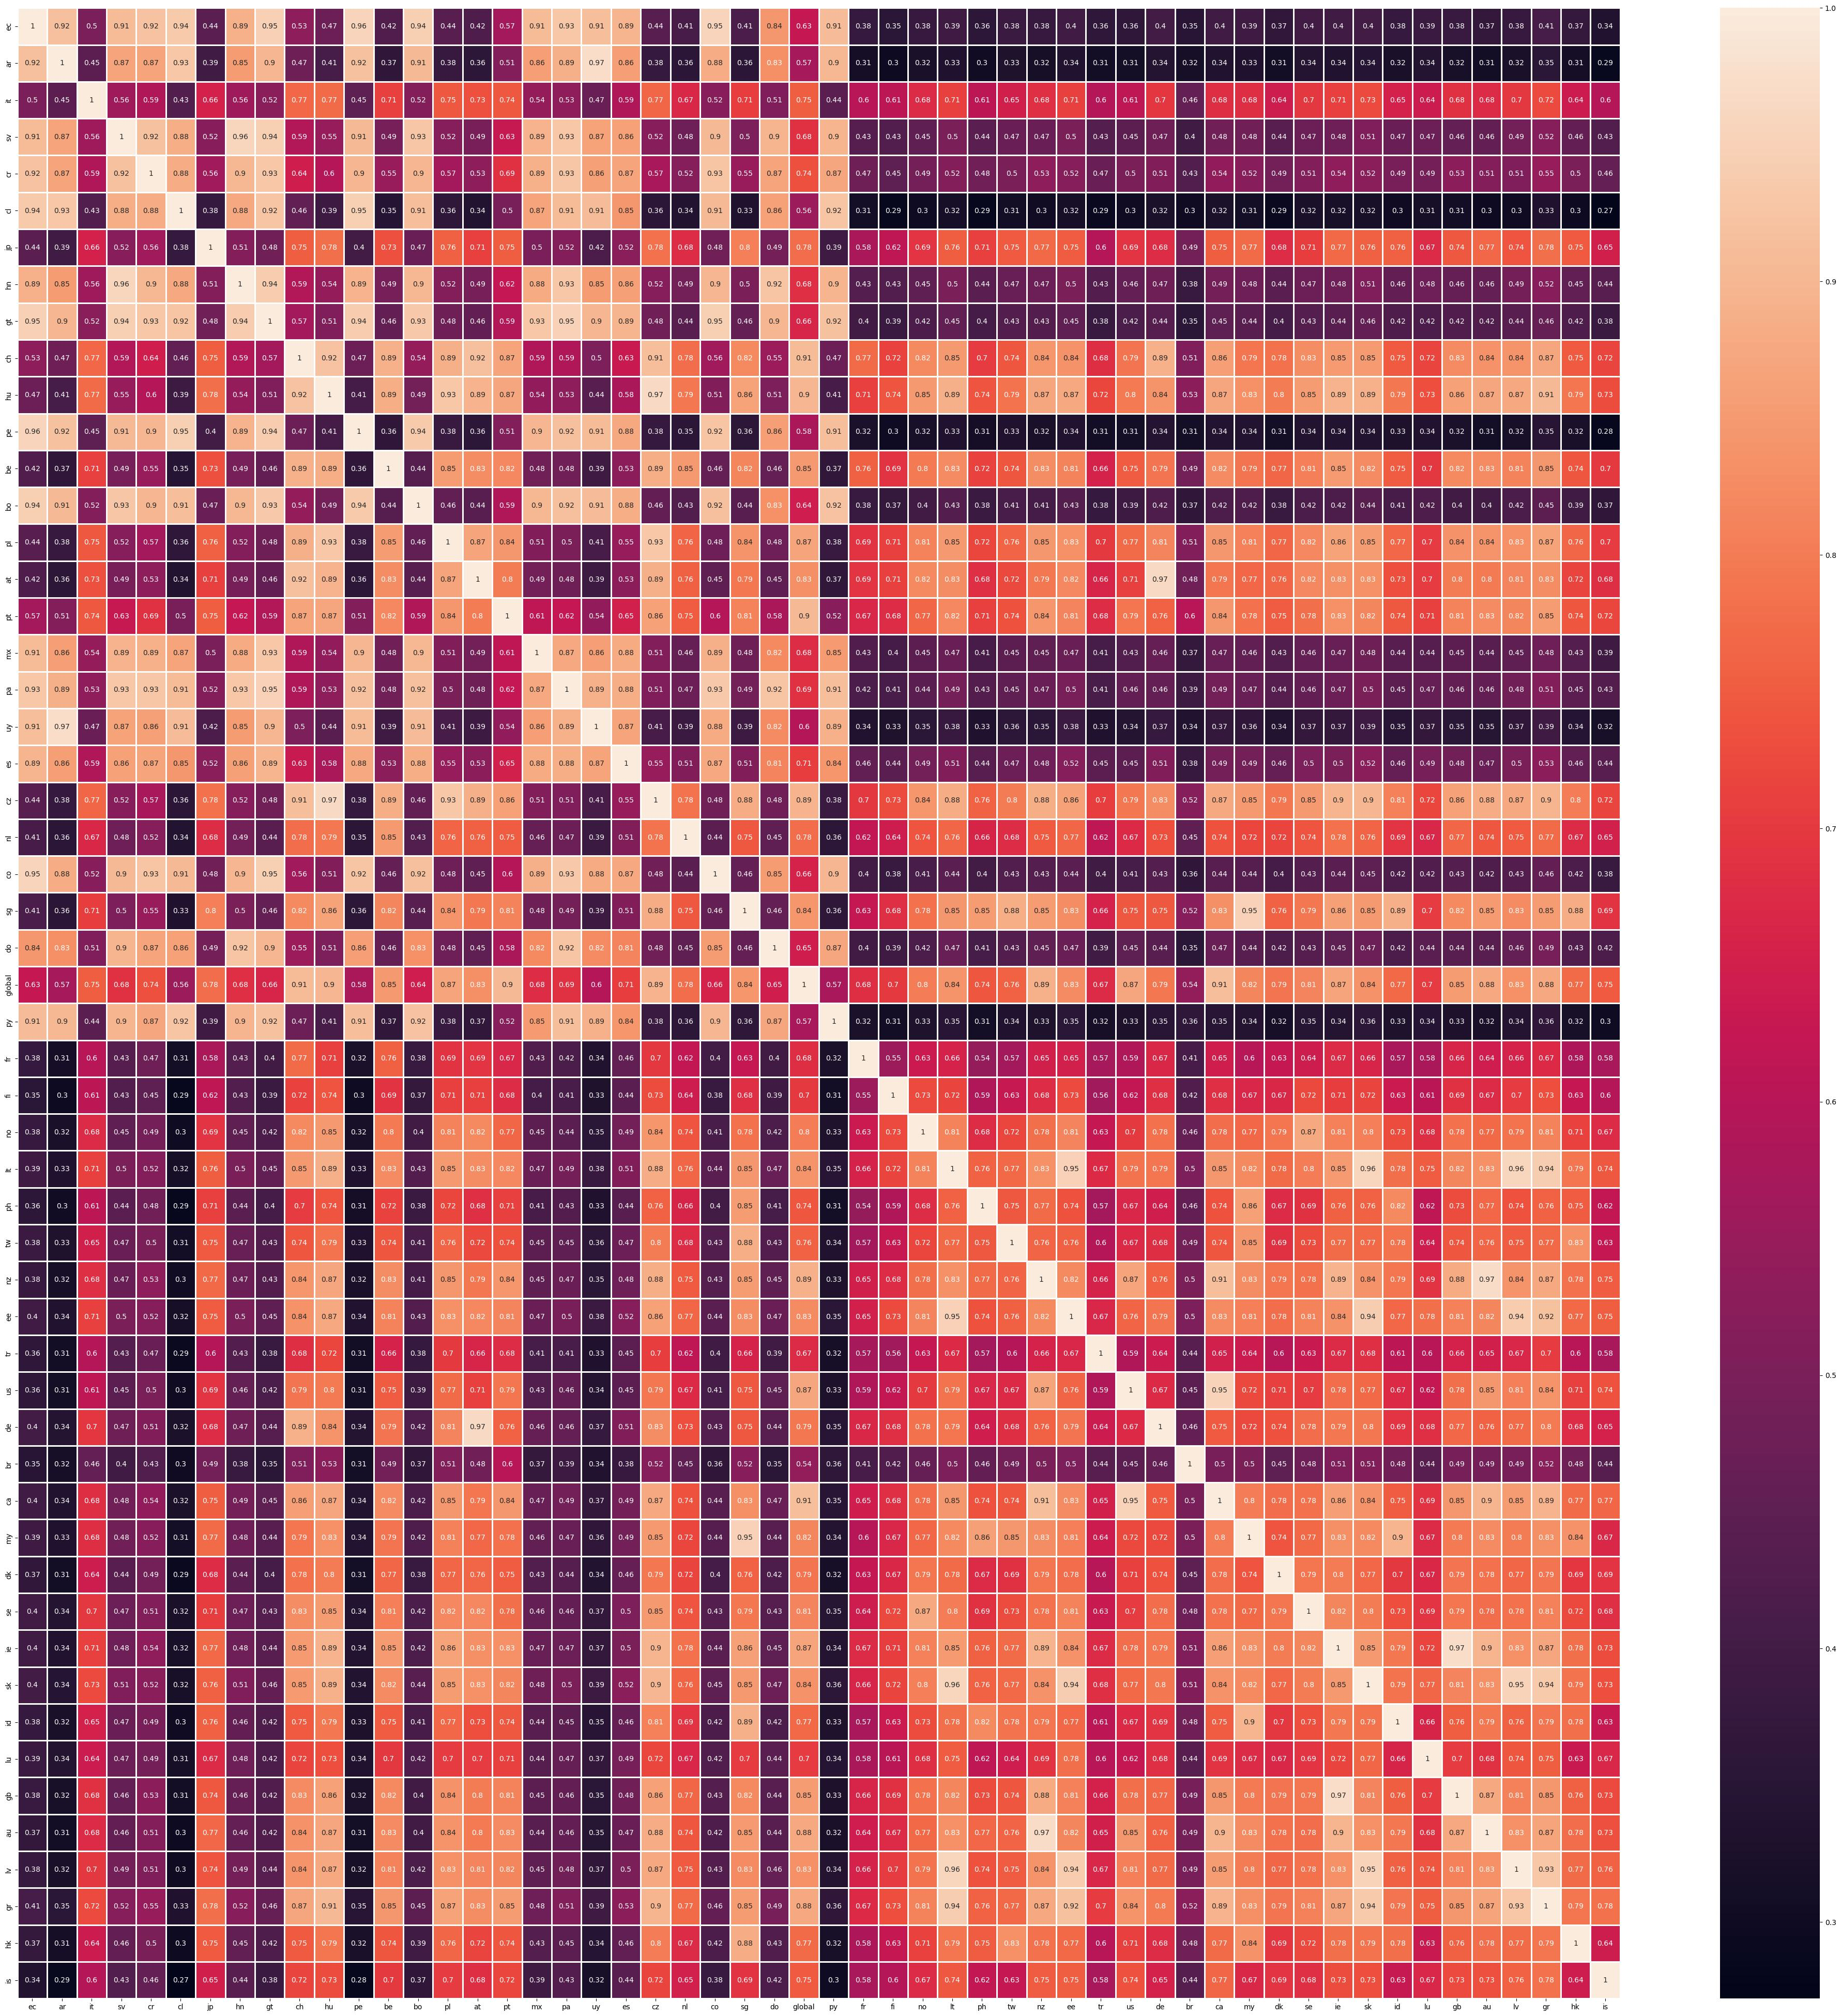
\includegraphics[scale = 0.19]{Figures/region_corr.jpeg}
    \caption{Correlation between popularity of track in different regions}
    \label{fig:corrRegion}
\end{figure} 
\label{appendix:a}







\end{document}



%%% Local Variables:
%%% mode: latex
%%% TeX-master: t
%%% End:
